\documentclass[tikz,border=3pt]{standalone}
\usetikzlibrary{decorations.pathmorphing}
\begin{document}
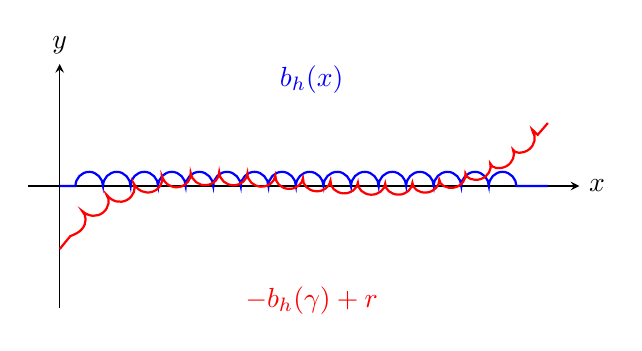
\begin{tikzpicture}[x=1cm,y=1cm,>=stealth]
  \draw[->] (-.4,0) -- (6.6,0) node[right] {$x$};
  \draw[->] (0,-1.55) -- (0,1.55) node[above] {$y$};
  \draw[blue,thick,decorate,
    decoration={bumps,segment length=7mm,amplitude=1.8mm,pre length=2mm,post length=2mm}]
    (0,0) -- (6.2,0);
  \draw[red,thick,decorate,
    decoration={bumps,segment length=7mm,amplitude=-1.5mm,raise=1mm,pre length=2mm,post length=2mm}]
    (0,-.8) .. controls (1.5,1.2) and (4.6,-1.2) .. (6.2,.8);
  \node[blue,above] at (3.2,1.05) {$b_h(x)$};
  \node[red,below] at (3.2,-1.15) {$-b_h(\gamma)+r$};
\end{tikzpicture}
\end{document}
